%%%%%%%%%%%%%%%%%%%% author.tex %%%%%%%%%%%%%%%%%%%%%%%%%%%%%%%%%%%
%
% sample root file for your "contribution" to a contributed volume
%
% Use this file as a template for your own input.
%
% SPRINGER  RECOMMENDED %%%%%%%%%%%%%%%%%%%%%%%%%%%%%%%%%%%%%%%%%%%%%%%%%%%
\documentclass[graybox]{svmult}

% choose options for [] as required from the list
% in the Reference Guide

\usepackage{mathptmx}       % selects Times Roman as basic font
\usepackage{helvet}         % selects Helvetica as sans-serif font
\usepackage{courier}        % selects Courier as typewriter font
\usepackage{type1cm}        % activate if the above 3 fonts are
                            % not available on your system
%
\usepackage{makeidx}         % allows index generation
\usepackage{graphicx}        % standard LaTeX graphics tool
                             % when including figure files
\usepackage{multicol}        % used for the two-column index
\usepackage[bottom]{footmisc}% places footnotes at page bottom

% see the list of further useful packages
% in the Reference Guide

\makeindex             % used for the subject index
                       % please use the style svind.ist with
                       % your makeindex program
%%%%%%%%%%%%%%%%%%%%%%%%%%%%%%%%%%%%%%%%%%%%%%%%%%%%%%%%%%%%%%%%%%%%%%%%%%%%%%%%%%%%%%%%%

% ADDED BY OURSELVES %%%%%%%%%%%%%%%%%%%%%%%%%%%%%%%%%%%%%%%%%%%%%%%%%%%
%% Package WE added
\usepackage[utf8]{inputenc}
\usepackage{hyperref}
\usepackage{xspace}
%% Definition WE made
\newcommand{\discovery}{DISCOVERY\xspace}
\newcommand{\ie}{\textit{i.e.}\xspace}
%% CT %%
\newcommand{\ftodo}[2][\relax]  % \TODO[editor]{text} 
  {\ensuremath{{}^{\mbox{\tiny\bf #1}}}~\textbf{#2}}


\begin{document}

\title*{Beyond The Clouds, How Should Next Generation Utility Computing Infrastructures Be Designed?}
\titlerunning{Beyond The Clouds, The \discovery Initiative}
% Use \titlerunning{Short Title} for an abbreviated version of
% your contribution title if the original one is too long
\author{Marin Bertier, Frédéric Desprez, Gilles Fedak, Adrien Lebre, Anne-Cécile
  Orgerie, Jonathan Pastor, Flavien Quesnel, Jonathan Rouzaud-Cornabas, Cédric Tedeschi}
\authorrunning{Lebre et al.} 
% Use \authorrunning{} for an abbreviated version of
% your contribution title if the original one is too long
%\institute{Name of First Author \at Name, Address of Institute, \email{name@email.address}
%\and Name of Second Author \at Name, Address of Institute \email{name@email.address}}
\institute{INRIA, France, \email{firstname.lastname@inria.fr}}
%
% Use the package "url.sty" to avoid
% problems with special characters
% used in your e-mail or web address
%
\maketitle

\abstract*{
%%% RR Proposal
%To accommodate the ever-increasing demand for Utility Computing (UC)
%resources, while taking into account both energy and economical issues, the 
%current trend consists in building larger and larger data centers in a few 
%strategic locations. Although such an approach enables to cope with the actual
%demand while continuing to operate UC resources through centralized software
%system, it is far from delivering sustainable and efficient UC infrastructures.
%%
%    We claim that a disruptive change in UC infrastructures is required: UC
%resources should be managed differently, considering locality as a primary
%concern. We propose to leverage any facilities available through the Internet
%in order to deliver widely distributed UC platforms that can better match the 
%geographical dispersal of users as well as the unending demand.  Critical to
%the emergence of such locality-based UC (LUC) platforms is the availability of
%appropriate operating mechanisms. In this paper, we advocate the implementation
%of a unified system driving the use of resources at an unprecedented scale by
%turning a complex and diverse infrastructure into a collection of abstracted
%computing facilities that is both easy to operate and reliable.
%%
%    By deploying and using such a \emph{LUC Operating System} on backbones, our
%ultimate vision is to make possible to host/operate a large part of the
%Internet by its internal structure itself: A scalable and nearly infinite set
%of resources delivered by any computing facilities forming the Internet,
%starting from the larger hubs operated by ISPs, government and academic
%institutions to any idle resources that may be provided by end-users.
%%
%    Unlike previous researches on distributed operating systems, we propose to
%consider virtual machines (VMs) instead of processes as the basic element.
%System virtualization offers several capabilities that increase the flexibility
%of resources management, allowing to investigate novel decentralized schemes.
%
%% Adrien's Proposal
%
Although the concept of Micro and Nano Data Centers (DCs) has been proposed to
deliver more efficient as well as sustainable Utility Computing (UC) resources,
the questions of where deploying and how federating thousands of such
facilities are still far to be solved and  the current trend of building larger
and  larger DCs in few strategic locations still prevails.
%
In this chapter, we claim that a new generation of UC platforms can be designed
by juxtaposing the concept of micro/nano DCs with the Internet backbone:
Instead of building and deploying dedicated facilities, we propose to  extend
each network point of presence with additional servers and to operate them
through a unified system in charge of turning a widely distributed
infrastructure into a collection of abstracted computing facilities that
natively matches the geographical dispersal of users. 
%
Unlike previous researches on distributed operating systems, we propose to
consider virtual machines (VMs) instead of processes as the basic element.
System virtualization offers several capabilities that increase the flexibility
of resources management, allowing investigating novel autonomic and
decentralized schemes.
}


%\abstract{Each chapter should be preceded by an abstract (10--15 lines long) that summarizes the content. The abstract will appear \textit{online} at \url{www.SpringerLink.com} and be available with unrestricted access. This allows unregistered users to read the abstract as a teaser for the complete chapter. As a general rule the abstracts will not appear in the printed version of your book unless it is the style of your particular book or that of the series to which your book belongs.\newline\indent
%Please use the 'starred' version of the new Springer \texttt{abstract} command for typesetting the text of the online abstracts (cf. source file of this chapter template \texttt{abstract}) and include them with the source files of your manuscript. Use the plain \texttt{abstract} command if the abstract is also to appear in the printed version of the book.}

%%%
\section{Context and Motivations\label{sec:intro}}

The success of Cloud Computing has driven the advent of Utility Computing. However, Cloud
Computing is a victim of its own success: In order to answer the escalating demand for
computing resources, Cloud Computing providers must build data centers~(DCs) of
ever-increasing size. Besides facing the well-known issues of large-scale platforms
management, large-scale DCs have to deal with energy considerations that limit the number
of physical resources that one location can host.

Instead of investigating alternative solutions that can tackle the aforementioned
concerns, the current trend consists in deploying larger and larger DCs in few strategic
locations presenting energy advantages. For example, Western North Carolina, USA, is an
attractive area due to its abundant capacity of coal and nuclear power following the
departure of the textile and furniture industry~\cite{greenpeace:2013}. More recently,
several proposals suggested building next generation DCs close to the polar circle in
order to leverage free cooling techniques, considering that cooling is accounting for a
big part of the electricity consumption~\cite{greenberg:sigcomm09}.

%%%
\subsection{Inherent Limitations of Large-scale DCs}

Although building large scale DCs  enables to cope with the actual demand,
% while continuing to operate UC resources through centralized software system 
it is far from delivering sustainable and efficient UC infrastructures. In addition to
requiring the construction and the deployment of a complete network infrastructure to
reach each DC, it exacerbates the inherent limitations of the Cloud Computing model:

\begin{itemize}
\item The externalization of private applications/data often faces legal issues that
  restrain companies from outsourcing them on external infrastructures, especially when
  located in other countries.
\item The overhead implied by the unavoidable use of the Internet to reach distant
  platforms is wasteful and costly in several situations: Deploying a broadcasting service
  of local events or an online service to order pizzas at the edge of the polar circle,
  for instance, leads to important overheads since most of the users are \emph{a priori}
  located in the neighborhood of the event/the pizzeria.
\item The connectivity to the application/data cannot be ensured by centralized dedicated
  centers, especially if they are located in a similar geographical zone. The only way to
  ensure disaster recovery is to leverage distinct sites.\footnote{``Amazon outages –
    lessons learned'',
    \href{http://gigaom.com/cloud/amazon-outages-lessons-learned/}{http://gigaom.com/cloud/amazon-outages-lessons-learned/}
    (valid on Nov 2013, the 30\textsuperscript{th}).}
\end{itemize}

The two first points could be partially tackled by hybrid or federated Cloud
solutions~\cite{armbrust:2010}, that aim at extending the resources available on one Cloud
with those of another one; however, the third one requires a disruptive change in the way
UC resources are managed.
%Deploying a local events broadcasting service or an
%online service to order pizza at the edge of the polar circle for instance, leads to an important overhead
%in terms of energy footprint, network exchanges as well as latency since it can be assumed
%that a vast majority of the users are located in the neighborhood of the event/the
%pizzeria.

Another issue is that, according to some projections of a recent IEEE
report~\cite{ieeenetreport:2012}, the network traffic continues to double roughly each
year. Consequently, bringing the IT services closer to the end-users is becoming crucial
to limit the energy impact of these exchanges and to save the bandwidth of some
links. Similarly, this notion of locality is also critical for the adoption of the UC
model by applications that need to deal with a large amount of data as getting them in and
out actual UC infrastructures may significantly impact the global
performance~\cite{Fos11}.

The concept of micro/nano DCs at the edge of the backbone~\cite{greenberg:sigcomm09} may
be seen as a complementary solution to hybrid platforms in order to reduce the overhead of
network exchanges. However, operating multiple small DCs breaks in somehow the idea of
mutualization in terms of physical resources and administration simplicity, making this
approach questionable.
% Moreover, the number of such micro/nano DCs will remain limited and the question of
% where and how federating a large number of such facilities are still not solved.

%%%
\subsection{Ubiquitous and Oversized Network Backbones}

One way to partially solve the mutualization concern enlightened by the defenders of
large-scale DCs is to directly deploy the concept of micro/nano DCs upon the Internet
backbone. People are (and will be) more and more surrounded by computing resources,
especially those in charge of interconnecting all IT equipments. Even though these small
and medium-sized facilities include resources that are barely
used~\cite{Andrew:2003,Benson:2010}, they can hardly be removed (\textit{e.g.} routers).
Considering this important aspect, we claim that a new generation of UC platforms can be
delivered by leveraging existing network centers, starting from the core nodes of the
backbone to the different network access points in charge of interconnecting public and
private institutions. By such a mean, network and UC providers would be able to mutualize
resources that are mandatory to operate network/data centers while delivering widely
distributed UC platforms that can better match the geographical dispersal of users.
%
% TODO: AL -> ACO, please introduce this point latter in the chapter
% As a consequence, several initiatives started investigating how they could be
%better leveraged to support the requirements and constraints of current IT
%usages.  The concept of \emph{data furnaces} \cite{liu:hotcloud11} is one of
%the promising idea that seeks to mitigate the cost of operating
%network/computing resources by using them as a source of heat inside public
%buildings such as hospitals or universities. 
%
Figure~\ref{fig:renater} allows to better capture the advantages of such a proposal.
%\ftodo[FQ$\rightarrow$ALL]{Nous n'avons pas encore introduit la contribution à ce stade $\rightarrow$ enlever cette phrase~?}
% We did, cf. above : WE CLAIM
It shows a snapshot of the network weather map of
RENATER\footnote{\href{http://www.renater.fr}{http://www.renater.fr}}, the backbone
dedicated to universities and research institutions in France. It reveals several
important points:
\begin{figure}[b]
\vspace*{-.3cm}

\includegraphics[width=10cm]{./FIGS/renater.png}
\centering\caption{The RENATER Weather Map on May 2013, the 27th, around 4PM.
Each red square corresponds to a particular point of presence (PoP) of the network. The map is available in real-time
at: \href{http://www.renater.fr/raccourci}{http://www.renater.fr/raccourci}}
\label{fig:renater}
\vspace*{-.3cm}
\end{figure}


\begin{itemize} 
\item As mentioned before, most of the resources are under-used (only two links are used
  between 45\% and 55\%, a few between 25\% and 40\%, and the majority below the threshold
  of 25\%).
\item The backbone was deployed and is renewed to match the demand: The density of points
  of presence~(PoP, \ie a small or medium-sized network centers) as well as the bandwidth
  of each link are more important on the edge of large cities such as Paris, Lyon or
  Marseille.
\item The backbone was designed to avoid disconnections, since 95\% of the PoPs can be
  reached by at least two distinct routes.
\end{itemize}


%\ftodo[AL -> ALL]{It might make sense to talk of congestion effects that we can see in Marseille and Paris, the two path to the rest of Internet.}

\subsection{Locality-based Utility Computing}

%This chapter aims at introducing a new generation of UC platforms that can be
%seen somehow as an extension of the concept of micro DCs. The main change is to
%consider locality as a key point of UC services and to leverage facilities
%composing the internet backbone.  %Instead of building and deploying dedicated
%facilities, we claim that next UC
%infrastructures should be tightly coupled with any facilities available through
%the Internet, starting from the core routers of the backbone, the different
%network access points and any small and medium-size computing infrastructures
%that may be provisioned by public and private institutions. 

% Although it involves radical changes in the way
%physical and virtual resources are managed, locating and operating computing
%power and data on
%facilities close to the end-users will deliver highly efficient
%and sustainable UC services, resolving inherent limitations of the cloud computing model leveraging large-scale DCs. 

This chapter aims at introducing locality-based UC infrastructures, a new generation of UC
platforms that solves inherent limitations of the Cloud Computing paradigm relying on
large-scale DCs. Although it involves radical changes in the way physical and virtual
resources are managed, leveraging network centers is a promising way to deliver highly
efficient and sustainable UC services.

From the physical point of view, network backbones 
%such as National Research and Educational Networks (NRENs) 
provide appropriate infrastructures, \ie, reliable and efficient enough to operate UC
resources spread across the different PoPs. Ideally, UC resources would be able to
directly take advantage of computation cycles available on network active devices,
\textit{i.e.} those in charge of routing packets. However, leveraging network resources to
make external computations may lead to important security concerns. Hence, we propose to
extend each PoP with a number of servers dedicated to VMs hosting. Because it is natural
to assume that the network traffic and UC demands are proportional, larger network centers
will be completed by more UC resources than the smaller ones. Moreover, by deploying UC
services on relevant PoPs, a LUC infrastructure will be able to natively confine network
exchanges to a minimal scope, minimizing both the energy footprint of the network, the
impact on latency and the congestion phenomena that may occur on critical paths (for
instance Paris and Marseille on RENATER).

From the software point of view, the main challenge is to design a complete distributed
system in charge of turning a complex and diverse network of resources into a collection
of abstracted computing facilities that is both reliable and easy to operate.

\begin{svgraybox}
  The design of the \emph{LUC  Operating System},  an advanced system being able to unify many UC
  resources distributed on distinct sites,  would enable Internet service providers~(ISPs)
  and other institutions in charge of operating a network backbone to build an
  extreme-scale LUC infrastructure with a limited additional cost. Instead of redeploying
  a complete installation, they will be able to leverage IT resources and specific devices
  such as computer room air conditioning units, inverters or redundant power supplies
  already present in each center of their backbone.
\end{svgraybox}


\medskip
%This chapter  describes  how such a new
%generation of highly efficient and sustainable UC can emerge through an integrated
%system, \ie the \emph{LUC Operating System}, leveraging advanced and P2P system mechanisms.

In addition to considering \emph{locality} as a primary concern, the novelty of the LUC OS
proposal is to consider the VM as the basic object it manipulates.  Unlike existing
research on distributed operating systems designed around the process concept, a LUC OS
will manipulate VMs throughout a federation of widely distributed physical
machines. Virtualization technologies abstract out hardware heterogeneity, and allow
transparent deployment, preemption, and migration of virtual environments~(VEs), \ie a set
of interconnected VMs.  By dramatically increasing the flexibility of resource management,
virtualization allows to leverage state-of-the-art results from other distributed systems
areas such as autonomous and decentralized systems.  Our goal is to build a system that
allows end-users to launch VEs over a distributed infrastructure as simply as they launch
processes on a local machine, \ie without the burden of dealing with resources
availability or location.

\subsection{Chapter Outline} 
Section~\ref{sec:challenges} describes the key objectives of a LUC OS and the associated
challenges.  Section~\ref{sec:background} explains why our vision differs from actual and
previous UC solutions. In Section~\ref{sec:archi}, we present how such a unified system
may be designed by delivering the premises of the \discovery system, an agent-based system
enabling distributed and cooperative management of virtual environments over a large-scale
distributed infrastructure.  Future work as well as opportunities are addressed in
Section~\ref{sec:future}. Finally Section~\ref{sec:conclusion} concludes this chapter.

%%%
\section{Overall Vision and Major Challenges\label{sec:challenges}}

Similarly to traditional operating systems (OSes), a LUC OS will be composed of a
significant number of mechanisms. Trying to identify all of them and establishing how they
interact is an on-going work (see Section~\ref{sec:archi}). However, having in
mind the goal of delivering a unified system in charge of operating a complex and diverse
infrastructure, and transform it into a LUC platform, we have identified the following
objectives to be considered when designing a LUC OS:

\begin{itemize} 
\item Scalability: a LUC OS must be able to manage hundreds of
  thousands of virtual machines (VMs) running on thousands of 
  geographically distributed computing resources, including small and
  medium-sized computing facilities as well as any idle resource that their owner would make available. These resources might be
  highly volatile, especially if the LUC infrastructure allows to include resources hosted by
  end-users.
\item Reactivity: To deal with the dynamicity of the infrastructure, a LUC OS
  should swiftly handle events that require performing particular
  operations, either on virtual or on physical resources, with the
  objective of maximizing the system utilization while meeting QoS expectations of VEs. 
  Reconfiguring  VEs over distributed resources, sometimes spread across wide area networks, or moving VMs, 
  while preserving their active connections, are examples of operations that should be performed as fast as possible.
\item Resiliency: In addition to the inherent dynamicity of the
  infrastructure, failures and faults should be considered as the norm rather than the
exception at such a scale. The goal is therefore to transparently leverage the
underlying infrastructure redundancy to (i)~allow the LUC OS to keep
working despite node failures and network disconnections and to (ii)~provide
snapshotting as well as high availability mechanisms for VEs.

\ftodo[CT (+FQ)$\rightarrow$AL]{les points (i) et (ii) ne sont pas indépendants, j'ai
  l'impression que pour résoudre le point (i), on va utiliser ce que tu
  mentionnes dans le point (ii), du coup, c'est pas vraiment une énumération.}

\item Sustainability: Although the LUC approach natively reduces the energy
footprint of UC services by minimizing the network impact, 
\ftodo[FQ$\rightarrow$AL]{Ce n'est pas l'avis du reviewer de Middleware. Et nous n'avons à ma connaissance 
pas de données pour affirmer une telle chose}
it is important to go one
step further by considering energy aspects at each level of a LUC OS
and propose advanced mechanisms in charge of an optimal usage of each source of energy. 
%Minimizing the energy footprint is a
%  transversal concern that has to be considered at each level of the
%  design of \discovery.
 To achieve such an objective, data related to the energy
  consumption of the VEs  and the computing resources
  as well as the environmental conditions (computer room air conditioning unit, location of the
  site, etc.) should be taken into account by the system.
\item Security and Privacy: Similarly to resiliency, security issues affect the LUC OS itself and the VEs running on it.
For the LUC OS security, the goals are to (i) create trust relationships between
different locations, (ii) secure the P2P layers, 
(iii) include security decision and enforcement points in the LUC OS and (iv) make them collaborate through the secured P2P layers to provide a secured infrastructure.
%  at different layers and locations to provide a end-to-end and in-depth security enforcement.
For the VEs security, we need to provide users with a way to express their security requirements that will be enforced by collaborating 
several LUC OS security decision and enforcement points.

\ftodo[AL/JP]{More on privacy? Only security is mentioned.}

\end{itemize}

In addition to the aforementioned objectives, targeting a distributed system
where VM is the elementary granularity requires to deal with important issues
regarding the management of the VM images. Managing VM images in a distributed
way across a WAN is a real challenge that will require to adapt
state-of-the-art techniques of replication and deduplication. Also,
several mechanisms of a LUC OS must take into account VM images'
location, for instance to allocate the right resources to a VE  or to request
VM images prefetching to improve deployment performance or VM relocations.

Amongst the numerous scientific and technical challenges that should be addressed, 
the lack of a global view of the system introduces a lot
of complexity. In order to tackle it while addressing the above-mentioned
challenges, we claim that internal mechanisms of a LUC OS should be based
on decentralized mechanisms specifically designed for it.
% the latest contributions in distributed and
% cooperative algorithms such as gossip-based approaches and self-* techniques.
These techniques should provide mechanisms which are fully decentralized and
autonomous, so to allow self-adapting control and monitoring of complex
large-scale systems. Simple locality-based actions by each of the entities
composing the system can lead to the global emergence of complex and
sophisticated behaviors, such as the self-optimization of resource allocation,
or the creation of decentralized directories. These techniques are starting to
be used in well-known large systems. As an example, the Amazon website relies on
its decentralized Dynamo service~\cite{decandia:2007} to create largely distributed indexes and recover from data
inconsistencies. Facebook’s Cassandra massive scale structured
store~\cite{lakshman:2010} also leverages P2P techniques for its core
operation.
%
In a LUC OS, decentralized and self-organizing overlays will enable to maintain
the information about
the current state of both virtual and physical resources, their characteristics and
availabilities. Such information is mandatory to build higher-level mechanisms ensuring the correct execution of VEs throughout 
the whole infrastructure. 
 
% To ensure scalability as well as flexibility, they should be constructed and operated using gossip-based techniques. 
%Considerable research needs to be conducted to provide core operating systems services in a
%fully decentralized way and without centrally maintained comprehensive knowledge of system's resources


%%%
\subsection{DVMS}\label{ssec:dvms}

%\subsubsection{Overview.}
DVMS~\cite{quesnel:ispa2013,quesnel:cpe2012} (Distributed Virtual Machine Scheduler) is a
framework that schedules VMs cooperatively and dynamically in large-scale distributed
systems. It is deployed as a set of agents that are organized following a ring topology
and that cooperate with one another to guarantee that VM demands are satisfied during
their executions. Concretely, when a node \footnote{In the following, 
\emph{node} and \emph{PM} will refer to the same entity (\emph{i.e} physical 
server of the infrastructure).} cannot guarantee the QoS for its hosted VMs or
when it is under-utilized, it starts an iterative scheduling procedure~(ISP) by querying
its first neighbor to find a better placement; it thus becomes the initiator of the ISP.
If the neighbor cannot satisfy the request, it is forwarded to the following free
node until the ISP succeeds. When a viable mapping has been found, the leader (\ie the last
peer that has taken part to the ISP) reconfigures the system by performing adequate VM
migrations. Such an approach allows each ISP to send requests only to a minimal number of
nodes and even though an ISP can reserve all nodes if the corresponding problem is
particularly hard to solve (thus guaranteeing that a solution will always be found if it
exits), experiments have shown that in most cases ISPs involve only few
nodes. Moreover, the DVMS proposal allows several ISPs to occur independently at the same
moment throughout the infrastructure; in other words, scheduling is performed on
partitions of the system that are created dynamically, which significantly improves the
reactivity of the system. To prevent conflicts that could occur if several ISPs performed
concurrent operations on the same PMs or VMs, it should be emphasized that PMs are reserved for
exclusive use by a single ISP.

An example involving three partitions is shown in Figure~\ref{fig:isp}; in particular, we
can see the growth of partition~1 between two steps. Explaining in detail the notion of
``first out'' is beyond the scope of this article but readers can consider that the
``first out'' relation enables to handle communications efficiently, as each node involved
in a partition can forward a request directly to the first node on the outside of its
partition~\cite{quesnel:cpe2012}.

\begin{figure}[h!]
  \centering
  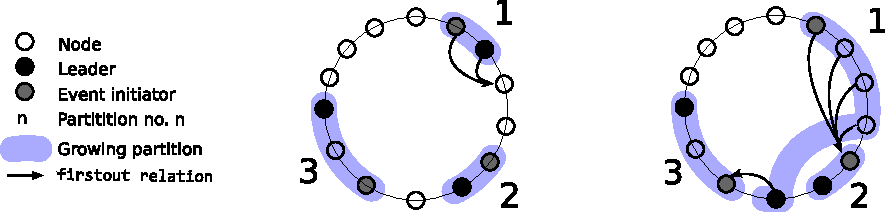
\includegraphics[width=0.9\linewidth]{Figures/resourceAcquisition-standard.pdf}
  \caption{Solving three problems simultaneously and independently with DVMS.}%
\small{The ring has been matched on top of three distinct clusters.}
  \label{fig:isp}%
\vspace*{-.3cm}
\end{figure}

We formally proved the correctness of DVMS using temporal logic, and we validated the first version of the prototype
at large scale (by means of simulations involving up to 80k VMs and 8k nodes and with experiments on the Grid'5000 testbed involving
up to 4.7k VMs and 470 nodes~\cite{quesnel:ispa2013}).

As discussed earlier, one limitation of this approach is related to its ring topology that
prevents it from taking into account the actual network topology.
%\subsubsection{Limitations of The Ring}
%
%Even though  DVMS can be deployed across several sites, it performs better on a
%cluster.
%
%The reason is simple.
%
%The ring is built without taking account of the network  topology; 
In other words, if the ISP strategy enables to limit the size of one partition to a
minimal number of nodes, these nodes are selected without considering the network
conditions at the time the ISP starts. This can lead to inefficient situations where VM
migrations occur between two nodes that are far from each other, which lasts longer than a
migration between two close nodes. Obviously the ring can be built to limit the
distance between peers globally (\ie peers of the same region/area would be grouped
together as illustrated in Figure~\ref{fig:isp}). However, in such a case, at least two
nodes of each group are directly connected to two far nodes.
%
Note that an approach such as the one proposed in~\cite{superchord}, which consists in
deploying one ring per site and relying on a \emph{super-ring}
to interconnect few representatives of each local ring, would not solve many
problems. Besides problems inherent to hierarchical and structured overlay networks, this
solution would not provide a good answer to locality: When going out of the local ring, it
would still not be possible to find the next closest ring.
%
%To sum up, the DVMS proposal lacks of a topology that can consider locality
%properties of a multi-sites infrastructure. 

% Autres limitations :
% -absence de tolerance aux pannes
% -peu d'evenements geres (surcharge d'un noeud)
% -ne prend pas en compte les liens entre VMS

\subsection{Overlay Networks and Locality}

As illustrated in the previous paragraph, one of the primary downsides of overlay networks
lies in that they break the physical topology by connecting nodes that have no physical
proximity.
%
Besides hierarchical attempts in building locality-aware overlay
networks~\cite{superchord,XuMK03,ECAN}, we can first mention the locality
improvement mechanisms of the Pastry structured overlay
network~\cite{pastry}. In order to reduce the latency of the routing process,
each node is given the opportunity to choose the closest nodes to fill its
routing table. Learning the existence of new nodes relies on a periodic exchange
of parts of routing tables.

Similar mechanisms have been adopted within unstructured overlay networks to make their
logical connections reflect the physical proximity of nodes, each node discovering its
closest nodes through gossiping. Note that the proximity between two nodes can be
estimated through any transitive metric, in particular the latency between the
nodes~\cite{tman}.

These approaches need to constantly maintain the knowledge of close nodes in order to
provide the \emph{best} node possible at the cost of periodic communications (uncorrelated
to the actual amount of requests to be processed by the overlay network).

The overlay network we propose in this paper differs in that it adopts a lazy approach consisting
in searching close nodes only upon receipt of requests. This way, the quality of the response
is proportional to the frequency of requests.

Our protocol relies on the Vivaldi protocol~\cite{dabek:2001:sigcomm04} to detect close
nodes. Vivaldi places nodes in a multi-dimensional space. Each node is given coordinates
inside this space reflecting its physical location. The protocol is based on simple
message exchanges. Initially, each node is given a random position in the space and
chooses (possibly arbitrarily) a small subset of nodes, composing its \emph{view}. Then,
each node starts estimating the round trip time between itself and another node chosen
randomly in its view, and adapts its distance with this node in the space accordingly,
coming closer to it or moving away from it. The nodes can repeat this step
independently (each with another node from its view), to improve the accuracy of the
positioning. A globally accurate positioning of nodes can be obtained very quickly (in a
small number of such steps) if nodes have a few long-distance nodes in their view and if the
network is not excessively dynamic. These long distance links can be easily maintained.

Recall that Vivaldi does not allow to directly know the nodes that are close in
the network, but to be able to recognize them through their coordinates. Our
overlay relies on the examination of Vivaldi coordinates of nodes discovered
during the processing of requests sent to it.







%%%
\section{Premises of a LUC OS: The \discovery Proposal\label{sec:archi}}

In this section, we propose to go one step further by discussing preliminary
investigations around the design and the implementation of a first LUC OS
proposal: the \discovery system (DIStributed and COoperative Management of
Virtual EnviRonments autonomouslY). We draw the premises of the \discovery
system by emphasizing some of the challenges as well as some research directions
to solve them. Finally, we give some details regarding the prototype that is
under development and how we are going to evaluate it.  

\subsection{Overview}

The \discovery system relies on a multi-agent peer-to-peer system deployed on
each physical resource composing the LUC infrastructure. Agents are autonomous
entities that collaborate to efficiently use the LUC resources. In our context,
efficiency means that a good trade-off is found between satisfying user's
expectations, ensuring reliability, reactiveness as well as availability of the
services while limiting the energy consumption of the system and providing
scalability. We propose thus to leverage P2P techniques, that
allow self-* properties, such as self-adaptation and self-repairing of overlays. 
%
To reduce the management complexity as well as the design and the
implementation of the different mechanisms that are mandatory, we strongly
support to use micro-kernel concepts. Such an approach should enable to design
and implement services at higher level while leveraging P2P mechanisms
at the lower ones.  Furthermore, to address the different objectives and reduce
the management complexity, we also underline that self-* properties should be
present at every level of the system.  We think that relying on a multi-agent
peer-to-peer system is the best solution to cope with the scale as well as the
network disconnections that may create temporary partitions in a LUC platform.

In \discovery, each agent has two purposes: (i) maintaining knowledge base on the
LUC platform composition (ii) ensuring the correct execution of the VEs. 
Concretely, the knowledge base will consist of overlays that will be used 
for the autonomous management of the
VEs life cycle. This includes the configuration, deployment and monitoring of
VEs as well as the dynamic allocation or relocation of VMs to adapt to changes
in VEs requirements and physical resources availability. To this end, agents
will need to rely on dedicated mechanisms that can be classified as follows: 

\begin{itemize}
\item Mechanisms related to physical resource localization and monitoring, 
\item Mechanisms related to VEs management, 
\item Mechanisms related to the VM images management, 
\item Mechanisms related to reliability,
\item Mechanisms related to security and privacy.
\end{itemize}

\subsection{Resource Localization and Monitoring Mechanisms\label{ssec:p2p}}

Keeping in mind that \discovery should be designed in a fully distributed way,
most of the mechanisms should build on top of overlays in order to abstract changes
that occur at the physical levels. The specific requirements of this platform
will lead to develop a particular kind of overlays, having minimalism in mind.

More concretely, the first step is to design, at the lowest level, a first
overlay layer intended to abstract out the details of the physical routes and
computing utilities, while satisfying the basic topology requirements needed --
locality and availability. This overlay needs to enable the communications
between any two nodes in the platform. While overlay computing has been
extensively studied over the last decade, we emphasize here on minimalism, and
one particular feature with regard to the envisioned platform described before:
retrieving physically close nodes from a given starting node.

\subsubsection*{Giving nodes a position}

The physical network's connections are considered as arbitrary. We choose to
rely on the Vivaldi protocol~\cite{dabek:2001:sigcomm04}. Vivaldi is a
distributed algorithms assigning coordinates in the plane to nodes of a
distributed systems, each node being equipped with a \emph{view} of the network,
\emph{i.e.}, a set of nodes it knows. This view is initially assumed as
arbitrary. Coordinates obtained by a node reflects its \emph{position} in the
network, \emph{i.e.}, close nodes in the network are given close coordinates in
the plane. This is achieved by every node periodically checking the round trip
time between itself and another node (from its view, a different one at each
step) and adapting its distance (by changing its coordinates) with this node in
the plane accordingly. 

\begin{figure}
  \begin{minipage}[c]{.45\linewidth}
	\vspace*{.5cm}
   \hspace*{-0.5cm}
      	\centering 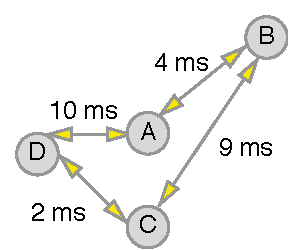
\includegraphics[width=4cm]{./FIGS/vivaldi_before.pdf}

   \hspace*{0.5cm}
	\vspace*{.4cm}
		\caption{Vivaldi plot before updating positions.}
		{\small Each node ping other nodes. Each node maintains a map of distance.}
\label{fig:vivaldi_before}
   \end{minipage}
\hspace*{0.6cm}
   \begin{minipage}[c]{.45\linewidth}
   	\centering 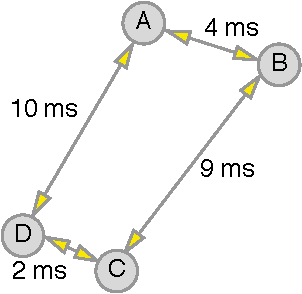
\includegraphics[width=4cm]{./FIGS/vivaldi_after.pdf}
	\vspace*{0.20cm}
		\caption{Vivaldi plot after updating positions.}
		\label{fig:vivaldi_after} 
{\small The computed positions of other nodes are periodically updated.}
  \end{minipage} \hfill
\end{figure}

\newpage

Note that a global accurate positioning of nodes can be
obtained if nodes have a few long-distance nodes in their
view~\cite{dabek:2001:sigcomm04}. These long distance links can be easily
maintained through a simple gossip protocol.

\subsubsection*{Searching for close nodes}

Once this map is achieved (each node its coordinates), we are able to decide
whether two nodes are close by calculating their distance. However, the view of
each node does not \emph{a priori} contain its closest nodes. We need additional
mechanisms to locate a set of nodes that are close to a given initial node --
Vivaldi gives a \emph{location} to a node, but not a neighborhood. To achieve
this, we use a modified distributed version of the classic Dijkstra's algorithms
used to find the shortest path between two nodes in a graph. The goal is to
build a \emph{spiral}\footnote{The term \emph{spiral} is here a misuse of
language, as there is no guarantee that the graph actually drawn in the plane
does not contain crossing edges. The only guarantee is that when following the
path constructed, the nodes are always further from the initial node.}
interconnecting the nodes in the plane that are closest to a given initial
node. Let us consider our starting point is node $s$. The first step is to find
a node to build a two-node spiral with $s$. Such a node is sought in the current
view of $s$ by selecting the node, say $a$, having the smallest distance with
$s$. By contacting $a$, $s$ then sends its view to $a$, $s$ stores $a$ as its
successor in the spiral, and $a$ adds $s$ as its predecessor in the spiral. Then
$s$ forwards its view to $a$. $a$ then creates a new view by keeping the $n$
node which are closest to $a$ in both $s$ and $a$'s views. This last view is
then referred to as the \emph{spiral view} and is intended to contain a set of
nodes in which to find the next step of the spiral. Then $a$ restarts the same
process: Among the spiral view, it chooses the node with the smallest distance
to $s$, say $b$, and adds it in the spiral -- $a$ becomes the predecessor of $b$
and $b$ becomes the successor of $a$. Then, the spiral view is sent to $b$ which
updates it with the nodes it has in its own view. The process is repeated until
we consider we have gathered enough nodes with regard to the requesting
application.

One risk to be mitigated is not to blocked by a spiral view containing only
nodes that are already in the spiral. However, this problem can be easily
addressed by forcing the presence of a few long distance nodes whenever it is
updated.

\subsubsection*{Learning}

Applying the protocol described above, the quality of the spirale is
questionable in the sense that the nodes that are actually close to the starting
point node $s$ may not be included. The only property ensured is that one step
forward the path built always takes us further from the starting point node.

To improve the \emph{quality} of the spiral, \emph{i.e.}, reduce the average
distance between the nodes it comprises and the initial node, we add a learning
mechanism coming with no extra communication cost, as it does not require any
extra message. When a node is contacted for becoming the next node in one
spiral, and receives the associated spiral view, it can also keep the nodes that
are closest to itself, thus potentially increasing the quality of a future
spiral construction.

\subsubsection*{Routing}

Still based on the minimal design, and independently from the spiral
constructions, there is a need for routing.

\ftodo[CT]{TODO}

% Each node doing so in parallel, a number of clusters are created inside which we
% can ensure a certain level of locality -- all nodes inside this group can
% communicate with each other very efficiently. Given the number of nodes in these
% groups, the inner topology of a group can either rely on very simple graphs,
% such as rings, or more connected graphs, to accelerate the dissemination and
% retrieval of information in the group. Note that, still based on simple
% gossiping techniques, such graphs can be easily maintained as the network's
% conditions change. For instance, if a link becomes overloaded, the other nodes
% will react to this change by removing nodes with which they communicate through
% this link from their local group. Such groups are exemplified on
% Figure~\ref{fig:renater_overlay} (for the west part of the platform).

% \begin{figure}[htbp]
% 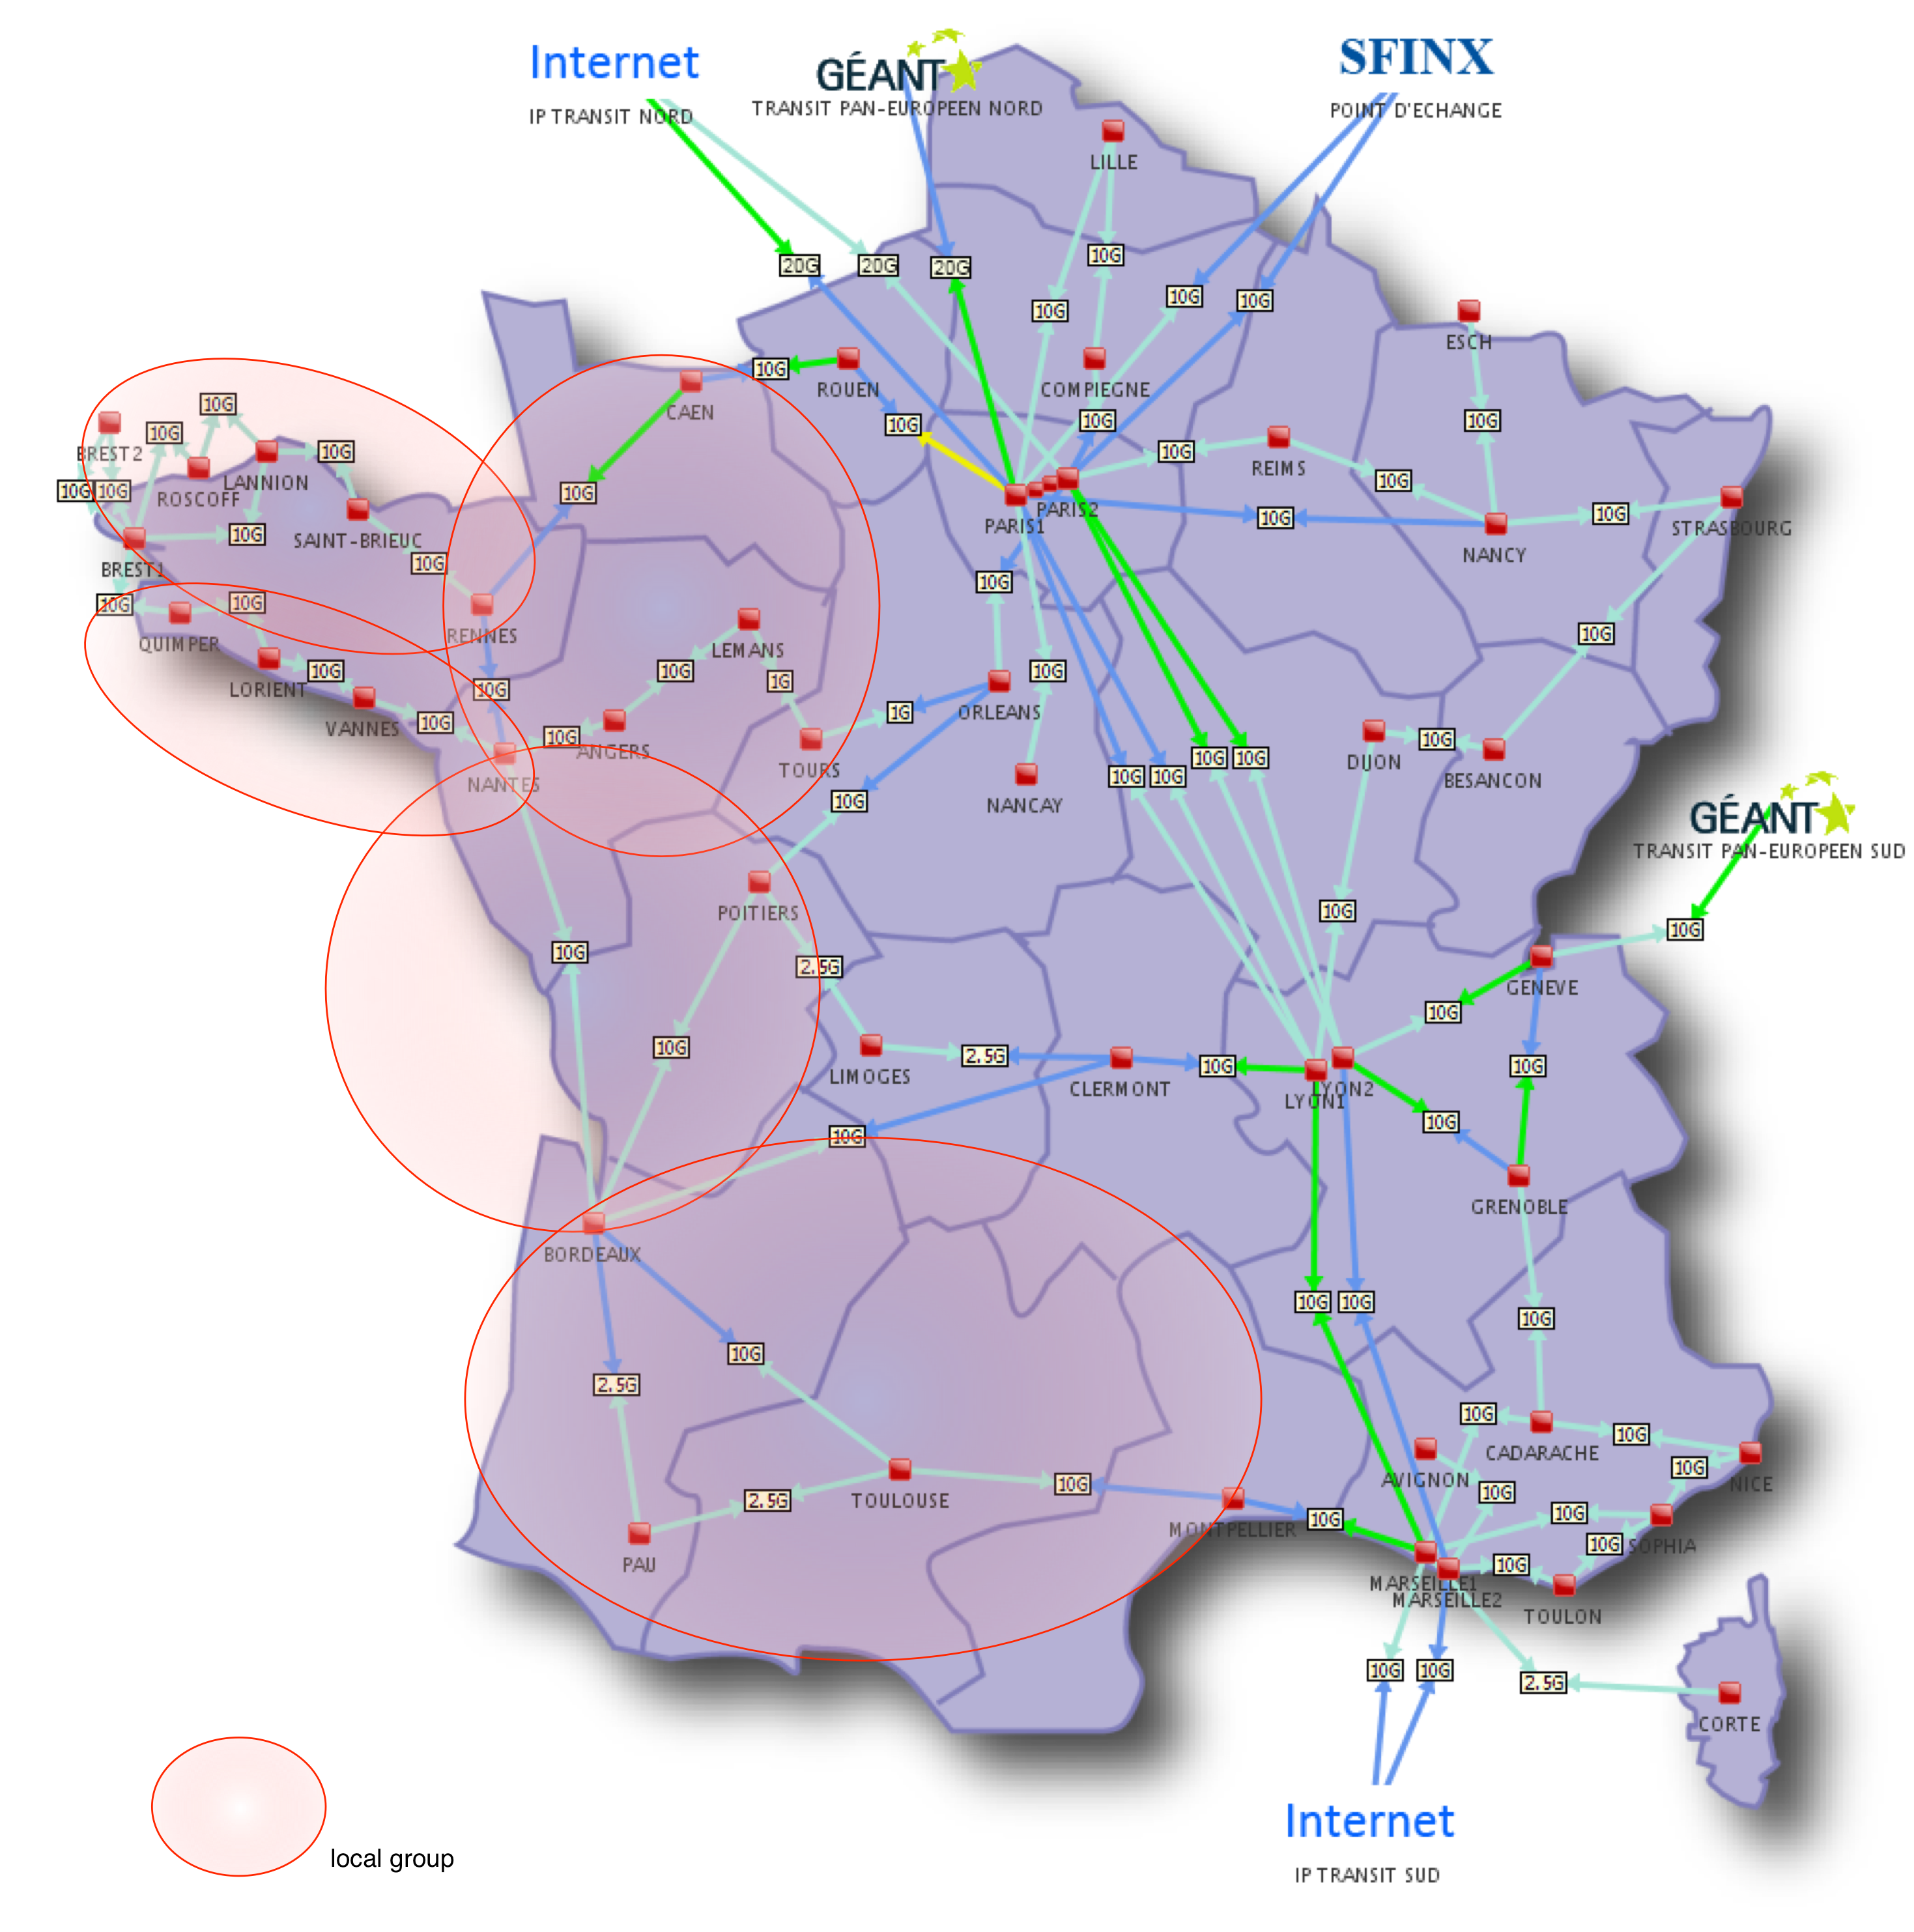
\includegraphics[width=12cm]{./FIGS/renater_overlay.png}
% \caption{Overlay local groups on top of the RENATER platform.\label{fig:renater_overlay}}
% \end{figure}

% As we can see on Figure~\ref{fig:renater_overlay}, it follows from the way the
% overlay is built that some nodes may be a member of several groups. The Nantes
% site for instance is part of three of these groups, given its
% physical position. More generally, the overlay will take the shape of a set of
% groups with some \emph{bridges} between the groups. Note that several
% \emph{bridges} can interconnect two local groups. Thus, any request first goes
% through local nodes allowing for its local processing, and avoiding the need for
% global coordination mechanisms.

% To be able to localize a particular VM, the system has to be able to route a
% request from any node to any other node. This functionality is the classic
% problem of P2P overlays, which is traditionally solved in structured overlay networks by
% maintaining a routing table on each node, and by a flooding mechanism or with
% random walks in unstructured overlays. These techniques are usually designed for
% very large scale networks with different guarantees and costs. Here, given the
% particular ``intermediate'' scale of the platform, and its specific
% requirements, we believe that these existing techniques are too
% \emph{powerful}. As we want to design a minimalistic overlay, there is room to
% try to design a new routing technique specifically fitting our
% requirements. The aim is then to maintain, in all groups, information about the
% distance between this group and \emph{close} groups in terms of number of bridge nodes
% to go through. Hence, the system will be able to route quickly between \emph{close}
% groups. The routing of requests between \emph{far} groups will be based on a random
% decision when no information are available, but \emph{oriented} by the aim of
% going away from the request's source.

% This overlay will provide the basic building block of the platform, on which will
% rely higher level overlays and functionalities, which are described in the
% following sections.

% \subsubsection*{Upper-Layer overlays}

% \ftodo[CT]{To be completed...}


% \ftodo[AL]{To be completed by Cedric and Marin}
% \ftodo[AL]{C/P from the proposal : 
% self-organizing overlay construction mechanisms based on gossip and epidemic
% techniques that will link the \discovery resources in navigable graphs onto
% which requests for VE can be routed and allocated. It will investigate
% mechanisms to quickly adapt these graphs to changing conditions and
% infrastructure, and mechanisms to monitor the adequacy of previous requests
% solutions to these changing conditions as these occur.}

\subsection{VEs Management Mechanisms}
\label{ssec:vem}
In the \discovery system, we define a VE as a set of VMs that may have specific
requirements in terms of hardware, software and also in terms of placement:~
some VMs must be on the same node/site in order to cope with performance objectives while
others should not be collocated in oder to ensure
high-availability criteria~\cite{hermenier:2013}.
As operations on a VE may occur in any place from any location, each agent should provide the capability
to configure and start a VE, to suspend/resume/stop it, to relocate some of its VM if need be or simply to retrieve the location of a particular VE. 
Most of these mechanisms are integrated on current UC platforms. However as mentioned, they
should be revisited to correctly run on the infrastructure we target
(\textit{i.e.} in terms of scalability, resiliency and reliability).
To this aim, the \discovery system relies on the aforementioned P2P mechanisms. 
As a first example, placing the VMs of a VE requires to be able to find available nodes that
fulfills the VM needs (in terms of resource needs as well as placement
constraints). Such a placement can start locally, close to the client
application requesting it, \textit{i.e.}, in its local group. If no such node is
found, simple navigation ensures that the request will encounter a bridge
eventually, leading to the exploration of further nodes. This navigation goes
on until one sufficiently available node is found.
A similar process is performed by the mechanism in charge of  dynamically
controlling and adapting the placement of VEs during their lifetime.  For instance, in
order to ensure particular needs of a VM, it can be necessary to relocate other
ones. According to the predefined constraints of VEs, some VMs might be
relocated on far nodes while other would prefer to be suspended.  Such a
mechanism has been deeply studied and validated in the DVMS
mechanism~\cite{dvms:wiki,quesnel:2012}. DVMS (Distributed Virtual
Machines Scheduler) enables to dynamically schedule a significant number of VMs
throughout a large-scale distributed infrastructure while guaranteeing VM
resource expectations.  

A second example regards the configuration of the network elements of a VE. 
Although it might look simple, assigning the right IPs to
each VM as well as maintaining the intra-connectivity of a VE becomes a bit more complex than in
the case of a single network domain, \textit{i.e.} a mono-site deployment.
%
Keeping in mind that a LUC infrastructure is
by definition spread WANwide, a VE can be hosted between distinct network
domains during its lifetime. No solution has been chosen yet. 
Our first investigations led us to leverage techniques
such as the IP over P2P project \cite{ganguly:2006}. However, the definition of
software network becomes more and more important. Investigating proposals such as
the Open vSwitch project \cite{pfaff:2009} looks a promising direction to solve such issue.
%

\subsection{VM Images Management}

In a LUC infrastructure, VM images could be deployed in any place from any
other location, but being in a large-scale, heterogeneous and widely spread
environment makes the management of VM images more difficult than more
conventional  centralized repositories.  
At coarse grain, the management of the VM images should be (i) consistent
with regards to the location of each VM throughout the \discovery infrastructure and
(ii) reachable in case of failures.
%
The envisioned mechanisms dedicated to the management of the VM images have been
classified into two sub-classes.
%
First, it will be mandatory to deliver appropriate mechanisms to efficiently
upload and replicate VM images among a high number of nodes in order to ensure
efficiency as well as reliability.  Second, the \discovery system should 
include specific mechanisms devoted to the scheduling of the VM image
transfers. Advanced policies are important to improve the efficiency of each
transfer that may occur either at the boot time or during VM relocations. 

Regarding storage and replication mechanisms,  an analysis of an IBM Cloud concludes
that a fully distributed model using P2P technology is not the best choice to manage VM images as the
number of instances of the same VM image is rather small~\cite{peng:2012}. However, central or
hierarchical solutions are not suited for the infrastructure we target.
Consequently, an augmented P2P solution working with replicas and
deduplication will have to be investigated in order to provide more
reliability, speed, and scalability to the system. For example, analyzing
different VM images shows that at least 30\% of the image is shared between
different VMs. This 30\% can become a 30\% space reduction, a
30\% increased reliability or a 30\% of speed increase. Depending on the
situation, we should decide to go from one scenario to another. 
%Finally, the number of replicas and deduplicated data should be dynamically balanced.

Regarding the scheduling mechanisms, it has been shown that a storage system with VMs being used by I/O intensive tasks 
can increase boot time from 10 to 240 seconds \cite{tan:2008}. Some actions like providing the
image chunks needed to boot first~\cite{tang:2011}, defining a new
image format, and pausing the rest of the I/O operations, can provide a
performance boost and limit the overhead that is still observed in commercial
Clouds~\cite{mao:2012}. 
%These actions should also take into account
%power-like metrics in order to reduce the energy consumption of data transfers.
%According to (Preist et Shabajee Nov 2010) the cost to transmit 1 MB can be of
%4Wh. Considering the size of VM images, any improvement aiming at reducing
%data movement will make a big difference.

More generally, the amount of data related to VM images is significant.
Actions involving data  should be aware of their implications on metrics like
(but not limited to): energy efficiency, bandwidth, reliability, proximity, and
hardware usage. The scheduler could also anticipate actions like moving images when
the load is low or the energy is cheaper.

%% \subsection{Reliability Mechanisms}
%% %These mechanisms should ensure  reliability and high availability of the
%% %\discovery system despite the scale and dynamicity of the underlying physical
%% %infrastructure.   
%% By nature, a LUC is a highly distributed platform where 
%% node and network failures will be much more frequent than in
%% actual UC platforms.  Furthermore, since resources could be located anywhere,
%% the expected mean time to repair failed equipments might be much larger than in
%% other platforms. For all these reasons, a set of dedicated mechanisms should be designed in order
%% to provide a fully transparent failure management with minimum downtime. 
%% %
%% To this aim, the \discovery system should include, first,  mechanisms in charge of its own reliability. 
%% Such mechanisms are required to avoid losing or corrupting important information
%% regarding the state of the system.  Of course, handling all kinds of failures
%% and implementing a fully resilient operating system is a complex task. Hence,
%% we propose to consider in a first time a crash-stop failure model. In other words, the
%% \discovery system should be able to autonomously restart any service by
%% relocating it on an healthy agent each time it is mandatory.  This implies to
%% define a common design pattern, \textit{i.e.} a set of recommendations, that each
%% service should follow to ensure such characteristics. Besides, in order to
%% ensure that such a pattern may be applied to stateful services, the system can
%% require a Cassandra like system \cite{lakshman:2010} that provides reliable and highly available
%% storage for critical system states. Retrieving the information related to one
%% service need to rely on the kind of mechanisms described in Section~\ref{ssec:p2p}.

%% %
%% In addition to be robust enough, the \discovery system should ensure the
%% reliable execution of virtual environments. The first mechanisms consists in
%% using snapshotting capabilities delivering by virtualization technologies.
%% Concretely, each internal states of a VM should be periodically saved on a
%% persistent storage.  When a crash occurs on a VM, its associated VE can be
%% restarted from the latest consistent states, \textit{i.e.} all VMs of the VE will be
%% resume for their latest snapshot.  As for the other mechanisms, performing VM
%% snapshotting in a large-scale, heterogeneous and widely spread environment is a
%% challenging task. However, we believe that aforementioned mechanisms in charge
%% of the VM images as well as recent proposals \cite{nicolae:2011} might enable
%% to provide such a feature. 
%% Although VM snapshotting provides a first level of reliability, it is not
%% sufficient to ensure high availability of the VE. More advanced mechanisms must
%% be proposed.  Our idea is to include mechanisms based on primary-backup
%% replication techniques. 
%% The basic principle is to have one active replica of the VM (the primary)
%% sending state updates to the other replicas (the backups) periodically. If the
%% primary fails, one of the backup can resume the execution transparently for the
%% outside world. Furthermore since the entire VM is replicated, applications can
%% be run unmodified.  Solutions to replicate VMs inside a cluster have been
%% proposed. However efficiently replicating VMs over a WAN is a huge challenge.
%% Limiting the size of the backup updates\cite{rajagopalan:2012}, and
%% reducing the impact of the required synchronizations on the execution of the
%% primary \cite{gerofi:2012}  are research directions to be further
%% studied. A better understanding of the parts of a VM that really need to be
%% updated is required. It might require to trade transparency for performance by
%% allowing latency-sensitive applications to define which part of their state has
%% to be updated.

%% \ftodo[AL]{Integrate the P2P aspect into the reliability section}
%% \subsubsection*{Monitoring Example}

%% Another key use of this low-level overlay is proactive replication of VMs,
%% keeping in mind that two identical VMs should be placed in relatively distant
%% nodes, for fault-tolerance reasons (close nodes have a high probability to fail
%% together). Following the defined overlay structure, this can be done through a
%% navigating scheme where at least one bridge is encountered. Monitoring this
%% replica can be done easily by having a \emph{watcher} in the same local group as
%% the replica.

\subsection{Reliability Mechanisms}
%These mechanisms should ensure  reliability and high availability of the
%\discovery system despite the scale and dynamicity of the underlying physical
%infrastructure.   
In a LUC, failures will be much more frequent than in actual UC
platforms. Furthermore, since resources could be highly distributed,
the expected mean time to repair failed equipments might be much
larger than in other UC platforms. For all these reasons, a set of
dedicated mechanisms should be designed in order to provide fully
transparent failure management with minimum downtime. 

%% It includes
%% mechanisms to ensure the high availability of the \discovery system
%% itself and mechanisms to allow executing VEs reliably.

Ensuring the high availability of the \discovery system requires being able to
autonomously restart any service by relocating it on a healthy agent each time
it is mandatory. To avoid losing or corrupting important information regarding
the state of the system, a Cassandra-like system~\cite{lakshman:2010} is
required to provide a reliable and highly available back-end for stateful
services.

Regarding VEs reliability, a first level of fault tolerance can be
provided by leveraging VMs snapshotting capabilities. Periodical
snapshots will allow restarting the VE from its last snapshot in the
event of a failure. Performing VM snapshotting in a large-scale,
heterogeneous, and widely spread environment is a challenging
task. However, we believe that adapting recently proposed
ideas~\cite{nicolae:2011} in this field would allow us to provide such
a feature.

Snapshotting is not enough for services that should be made highly
available, but a promising solution is to use VM
replication~\cite{Petrovic2012}. To implement VM replication in a WAN,
solutions to optimize synchronizations between
replicas~\cite{gerofi:2012,rajagopalan:2012} should be
investigated. Also, we think that a LUC has the major advantage over
other UC platforms, that it is tightly coupled with the network
infrastructure. As such, we can expect \emph{low} latencies between
nodes and so, to be able to provide strong consistency between
replicas while achieving acceptable response time for the replicated
services. 
%Note that the overlays presented in Section~\ref{ssec:p2p}
%for replicas localization and monitoring. Locating replicas based on a
%navigating scheme where at least one bridge is encountered, would be
%enough to ensure that they have a low probability to fail
%simultaneously.


Reliability techniques will of course make uses of the overlays
for resource localization and monitoring. 
Replicated VMs should be hosted on nodes that have a low
probability to fail simultaneously. Following the previously defined
overlay structure, this can be done through a navigating scheme where
at least one bridge is encountered. Monitoring a replica can then be
done by having a \emph{watcher} in the same local group as the
replica.

%% Another key use of this low-level overlay is proactive replication of VMs,
%% keeping in mind that two identical VMs should be placed in relatively distant
%% nodes, for fault-tolerance reasons (close nodes have a high probability to fail
%% together). Following the defined overlay structure, this can be done through a
%% navigating scheme where at least one bridge is encountered. Monitoring this
%% replica can be done easily by having a \emph{watcher} in the same local group as
%% the replica.




%
%% To this aim, the \discovery system should include, first,  mechanisms in charge of its own reliability. 
%% Such mechanisms are required to avoid losing or corrupting important information
%% regarding the state of the system.  Of course, handling all kinds of failures
%% and implementing a fully resilient operating system is a complex task. Hence,
%% we propose to consider in a first time a crash-stop failure model. In other words, the
%% \discovery system should be able to autonomously restart any service by
%% relocating it on an healthy agent each time it is mandatory.  This implies to
%% define a common design pattern, \textit{i.e.} a set of recommendations, that each
%% service should follow to ensure such characteristics. Besides, in order to
%% ensure that such a pattern may be applied to stateful services, the system can
%% require a Cassandra like system \cite{lakshman:2010} that provides reliable and highly available
%% storage for critical system states. Retrieving the information related to one
%% service need to rely on the kind of mechanisms described in Section~\ref{ssec:p2p}.

%% %
%% In addition to be robust enough, the \discovery system should ensure the
%% reliable execution of virtual environments. The first mechanisms consists in
%% using snapshotting capabilities delivering by virtualization technologies.
%% Concretely, each internal states of a VM should be periodically saved on a
%% persistent storage.  When a crash occurs on a VM, its associated VE can be
%% restarted from the latest consistent states, \textit{i.e.} all VMs of the VE will be
%% resume for their latest snapshot.  As for the other mechanisms, performing VM
%% snapshotting in a large-scale, heterogeneous and widely spread environment is a
%% challenging task. However, we believe that aforementioned mechanisms in charge
%% of the VM images as well as recent proposals \cite{nicolae:2011} might enable
%% to provide such a feature. 
%% Although VM snapshotting provides a first level of reliability, it is not
%% sufficient to ensure high availability of the VE. More advanced mechanisms must
%% be proposed.  Our idea is to include mechanisms based on primary-backup
%% replication techniques. 
%% The basic principle is to have one active replica of the VM (the primary)
%% sending state updates to the other replicas (the backups) periodically. If the
%% primary fails, one of the backup can resume the execution transparently for the
%% outside world. Furthermore since the entire VM is replicated, applications can
%% be run unmodified.  Solutions to replicate VMs inside a cluster have been
%% proposed. However efficiently replicating VMs over a WAN is a huge challenge.
%% Limiting the size of the backup updates\cite{rajagopalan:2012}, and
%% reducing the impact of the required synchronizations on the execution of the
%% primary \cite{gerofi:2012}  are research directions to be further
%% studied. A better understanding of the parts of a VM that really need to be
%% updated is required. It might require to trade transparency for performance by
%% allowing latency-sensitive applications to define which part of their state has
%% to be updated.

%% \ftodo[AL]{Integrate the P2P aspect into the reliability section}
%% \subsubsection*{Monitoring Example}

%% Another key use of this low-level overlay is proactive replication of VMs,
%% keeping in mind that two identical VMs should be placed in relatively distant
%% nodes, for fault-tolerance reasons (close nodes have a high probability to fail
%% together). Following the defined overlay structure, this can be done through a
%% navigating scheme where at least one bridge is encountered. Monitoring this
%% replica can be done easily by having a \emph{watcher} in the same local group as
%% the replica.


\subsection{Security and Privacy Mechanisms}
%
%LUC OS should include a mechanism for the security of the lower layers and particularly multiple P2P overlays.
%% Previous research~\cite{sybilattacks} has shown that without trusted identities, it 
%% is not possible to protect a P2P overlay against sybil attacks. 
%Recent advances~\cite{Castro:2002:SRS:844128.844156} in DHT 
%security might enable to provide a secured overlay. 
%But they are not sufficient to ensure the good behavior of resources and users.
%LUC OS should include an authentication and certification mechanism that 
%evaluates the behavior of resources and VEs.
%% Finally, as the resources could be hosted in more or less secured locations and provided by different 
%% resource providers, this certification should also be used to rank the security of each resources.
%% \ftodo[AL->JRC]{Could you please put only the most relevant one}
%
%Moreover, LUC OS shoud integrate security decision and enforcement points (SDEPs).
%%  mechanisms at all locations and layers.
%To guarantee a security, 
%Sandhu~\cite{sandhu_towards_2010} propose a roadmap towards such security mechanisms for
%Cloud where the Cloud infrastructure provides security hooks and
%mechanisms. 
%% To realize this goal, they point out the need for
%% \emph{developing models, methodologies and architectures for
%%   decentralized dynamic management of security and assurance
%%   policies}. 
%Similarly than other mechanisms, 
%As LUC infrastructure is even more distributed, heterogeneous and 
%dynamic than Cloud, its SDEPs should be distributed and 
%decentralized and able to evolve according to security requirements 
%without central security decision points. Futhermore, 
%LUC OS should provide a protocol to ease the collaboration between the SDEPs.
%Indeed, when new resources join
%a LUC infrastructure, SDEPs from different locations 
%must collaborate to extend the LUC infrastructure while keeping it secured. This collaboration between 
%SDEPs will also append when a VE is spread over different 
%resources and/or migrate from one to another.
%
%LUC OS should allow users to express their security requirements on their VEs.
%The expression of these requirements itself is a complex task.
%% LUC OS must propose to the user a way to model their VEs and 
%% the security requirements on them. 
%To ease the expression of these 
%requirements, LUC OS must propose a domain specific security language 
%that defines high-level security requirements such as \cite{rouzaud_book13b,Bacon:2010:EEA:2023718.2023739} do 
%for Clouds. These security requirements will be enforced 
%by SDEPs during the whole life time of the VE.
%
%%%%
% 1./ Securiser les overlays
% 3.a./ Definir  un DSL pour les VEs
% 3.b/ Offrir des moyens d'integrer des SDEPs (i.e. moulinette qui maintient/execute les DSLs)
% 2./ Securiser l'acces aux operations de manipulation de l'infra (admin et user)

% 1
To be successful, \discovery needs to provide mechanisms and methods to construct trust relationships between resource providers.
Trust relationships are known to be complex to build~\cite{Miller:2010:TWT:1907636.1907726}. Providing strong authentication, assurance and certification mechanisms for 
providers and users is required but it is definitely not enough. Trust covers socio-economic aspects that must be covered but are out of the scope of this chapter.
The challenge is to provide a trusted \discovery base.

% 2 
As overlays are fundamentals for all \discovery mechanisms, the first challenge is to ensure
that they are not compromise. Recent advances~\cite{Castro:2002:SRS:844128.844156} might enable to tackle such concerns.

%3.A ? 
The second challenge will consist in providing end-users with a way to define their own  security policies and to ensure that such policies are enforced. 
The expression of these requirements itself is a complex task.
The challenge is to improve the current trade-off between security and usability.
To ease the expression of these policies, we are currently defining a  domain specific security language
that defines high-level security requirements \cite{rouzaud_book13b,alefray:hpdc:2013}. 
These security policies will be enforced in a decentralize manner
by distributed security decision and enforcement points (SDEPs) during the whole lifetime of the VE.
Implementing such SDEP mechanisms in a distributed fashion will require to
conduct specific research as they are currently only prospective proposals for
classic UC infrastructures~\cite{Bacon:2010:EEA:2023718.2023739,sandhu_towards_2010}. 
The challenge will consist in investigating whether such proposals can be adapted to the LUC
infrastructure by leveraging appropriate overlays.
%%  

% Finally, as traditional distributed systems, \discovery should ensure the good behavior of resources and users.
% To this aim, authentication and certification mechanisms should be provided. 

\subsection{Toward a First Proof-of-Concept}

The first prototype is under heavy implementation. It aims at delivering a
simple mock-up for integration/collaboration purposes.  Following the
coarse-grained architecture described in the previous sections, we have
started to identify all the components participating in the system, their
relationships, as well as the resulting interfaces. 
Conducting such a work now is mandatory to move towards a more complete as well
as more complex system. 

To ensure a scalable and reliable design, we  chose to rely on the use
of high-level programming abstractions, more precisely, we are using distributed
complex event programming \cite{janiesch:2011} in association with actors
model \cite{agha:1986}. This enables to easily switch between a push and a pull
oriented model according to our needs. 
%To make the integration of the mechanisms easier, we propose to follow a Service
%Oriented Architecture \cite{valipour:iccsit09}.

Our preliminary studies showed that a common building block is mandatory to
handle resilience concerns in all components. Concretely, it corresponds to a
mechanism in charge of throwing notifications that are triggered by the low
level network overlay each time a node joins or leaves it.  Such a mechanism
makes the design and the development of higher building blocks easier as they do
not have to provide specific portions of code to monitor infrastructure
changes. 

This building block has been designed around the \emph{Peer Actor} concept (see~Figure~\ref{fig:supervisor} and
~\ref{fig:peeractor}).
 The \emph{Peer Actor} serves as an interface between higher services
and the communication layer. It provides methods that enable to define the behaviors of a
service when a resource joins or leaves a particular P2P overlay as well as
when neighbors change.
Considering that several overlays may co-exist through the \discovery system, 
the association between a \emph{Peer Actor} and its \emph{Overlay Actor} is
done at runtime and can be changed on the fly if need be. However, it is noteworthy that 
each \emph{Peer Actor} takes part to one and only one overlay at the same time.  
%
In addition to the \emph{Overlay Actor}, a \emph{Peer Actor}  is composed of a
\emph{Notification Actor}  that processes events and notifies registered actors.
%
As illustrated in Figure~\ref{fig:peeractor}, a service can use more than one \emph{Peer Actor} (and reciprocally). 
Mutualizing a \emph{Peer Actor} enables for instance to reduce the network overhead implied by the overlays' maintenance. 
In the example, the first service relies on a \emph{Peer Actor} implementing a Chord
overlay while the second service uses an additional \emph{Peer Actor} implementing a CAN structure.
 
\begin{figure}
  \begin{minipage}[c]{.35\linewidth}
	\vspace*{.5cm}
   \hspace*{-0.5cm}
      	\centering 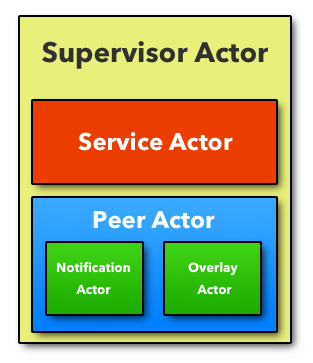
\includegraphics[width=4cm]{./FIGS/these_supervisor.png}

   \hspace*{0.5cm}
	\vspace*{.4cm}
		\caption{The Peer Actor Model}
		{\small The Supervisor actor monitors all the actors it encapsulates while the Peer actor acts as an interface between the services and the overlay.}
\label{fig:supervisor}
   \end{minipage}
\hspace*{0.6cm}
   \begin{minipage}[c]{.55\linewidth}
   	\centering 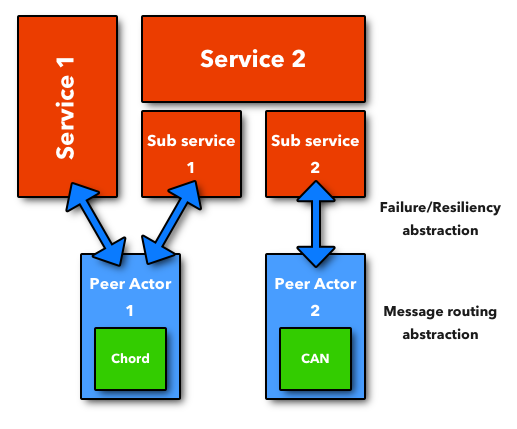
\includegraphics[width=6.5cm]{./FIGS/these_service_peer_archi_legend.png}
	\vspace*{-0.25cm}
		\caption{A Peer Actor Instantiation}
		\label{fig:peeractor} 
{\small The first service relies on a \emph{Peer Actor} implementing a Chord
overlay while the second service uses an additional \emph{PeerActor} implementing a CAN structure.}
  \end{minipage} \hfill
\end{figure}

By such a mean, higher-level services can take the advantage of the advanced
communication layers without dealing with the burden of managing the different
overlays. As an example, when a node disappears, all services that
have been registered as dependent on such an event are notified. 
Service actors can thus react accordingly to the behavior that has been specified. 
%
%Finally, to ensure the reliable execution of the different actors, each one is supervised by a parent entitled 
%the {Supervisor Actor} (see Figure \ref{fig:SupervisorActor}).
%
%
% we consider that at this scale, failures are the norm
%rather than the exception, so we decided that each actor will be monitored
%by a \emph{Supervisor actor}. \discovery services are under the supervision of the
%\
%
%: an actor may crash for a variety of reasons
% we decided that each of the system's actors will be
%supervised by a parent actor called \emph{Supervisor actor} (figure 
%\ref{fig:SupervisorActor}): an actor may crash for a variety of reasons
%(network disruption, byzantine failure, etc.) and it is normal to consider that
%different kind of failures can lead to different reactions of the system. These 
%reactions will be decided by the \emph{Supervisor actor}: reboot of the actor,
%escalation of the error, etc.

Regarding the design and the implementation of the \discovery system, each
service is executed inside its own actor and communicates by
exchanging messages with the other ones. This ensures that each
service is isolated from the others : When a service crashes and needs to be
restarted, the execution of other services is not affected. 
% Besides, each service will be supervised by a global actor that encapsulates all
% services, ie. the \discovery agent. Each time a service fails, the \discovery
% agent catches and analyzes the failure so that it can decide which operations
% to perform. 
%
As previously mentioned, we consider that at the LUC scale, failures are the norm
rather than the exception, hence we decided that each actor will be monitored
by a \emph{Supervisor Actor} (see Figure~\ref{fig:supervisor}). \discovery services are under the supervision of the \discovery agent: this design makes it possible to precisely define strategy
that will be executed in case of service failures. This will be the way we
introduce self-healing and self-organizing properties to the \discovery system.

This building block has been fully implemented\footnote{Code is available at:
\href{https://github.com/BeyondTheClouds}{\url{https://github.com/BeyondTheClouds}}} by 
leveraging the SCALA/akka\footnote{\href{http://www.akka.io}{\url{http://www.akka.io}}} framework.

As a proof of concept, we are implementing a first high level service in charge
of dynamically scheduling VMs across a LUC infrastructure by leveraging the
DVMS~\cite{quesnel:2012} proposal (see Section \ref{ssec:vem}). The low-level
overlay that is currently implemented, is a robust ring based on the  Chord  algorithm. 

% When a node cannot guarantee the QoS for its
%hosted VMs, it starts an iterative scheduling procedure (ISP) by querying its
%neighbor to find a better placement. If the request cannot be satisfied by the
%neighbor (i.e., there is no viable placement to ensure the QoS of all VMs
%hosted on both reserved nodes), the request is forwarded to the following free
%node that takes part in that ISP.  The `absorption' of a new node is repeated
%until the ISP succeeds.  This approach allows DVMS to consider only a minimal
%number of nodes, thus decreasing the scheduling time without requiring a
%central coordinator.  Moreover, it allows several ISPs to occur independently
%at the same moment throughout the infrastructure.  To prevent deadlocks that
%may occur when all nodes are reserved by active ISPs, a distributed deadlock
%prevention mechanism has been designed. It enables DVMS to merge pairs of
%partitions.  To sum things up, the DVMS proposal has been designed to be fully
%distributed, non-predictive and event-driven by using partial views of the
%system.  Such a mechanism perfectly fits the requirements of a LUC OS.  The
%missing part was to extend DVMS in order to take into account resiliency
%aspects. This is going to be solved as we are implementing the DVMS algorithm
%with the \emph{Peer Actor}. 
%

To validate the behavior, the performance as well as the reliability of our
POC, we rely first on the Simgrid~\cite{Casanova:2008:SGF:1397760.1398183}
toolkit. Simgrid has been recently extended to integrate virtualization abstractions and accurate migration models. 
Simulations enable us to analyze particular situations and get several metrics
that cannot be easily monitored  on a real platform.
Second, results obtained from simulations are then compared to real experiments on the Grid'5000 platform. 
Grid'5000 provides a testbed supporting experiments on various types of
distributed systems (high-performance computing, grids, peer-to-peer systems,
Cloud Computing, and others), on all layers of the software stack. The core
testbed currently comprises 10 sites geographically spread across France. 
For the Discovery purpose, we developped a set of scripts that enables to deploy in a \emph{one-click} fashion a large number of VMs throughout 
the whole infrastructure\cite{flauncher}. By deploying our POC on each node and by
leveraging the VM deployment scripts, we can evaluate real scenario usages by conducting specific workloads in the different VMs. 
The validation of this first POC is almost completed. 
The resulting system will be the first to provide reactive,
reliable and scalable
reconfiguration mechanisms of virtual machines in a fully distributed and
autonomous way. This new result will pave the way for a complete proposal of
the \discovery system. 




%%%
\section{Future Work/Opportunities\label{sec:future}}

%\subsection{How Evaluating LUC proposals}
%
%We first need to evaluate the quality of our LUC design in terms of performance and fault
%tolerance. For such a large system over a wide infrastructure, getting an analytical model
%is indeed a tough task. To make sure that the overall systems is efficient and reliable,
%simulation and experimentation over an actual platform are the best way to evaluate it. We
%will first rely on simulation to validate independent parts of the overall
%system. Simgrid~\cite{Casanova:2008:SGF:1397760.1398183} will be our platform
%of choice for this evaluation. We are currently adding virtualization
%simulation capabilities to the simulator. Our second evaluation platform will
%be Grid'5000. It provides a testbed supporting experiments on various types of
%distributed systems (high-performance computing, grids, peer-to-peer systems,
%cloud computing, and others), on all layers of the software stack. The core
%testbed currently comprises 10 sites. 
%%Grid'5000 is composed of almost 8000 CPU cores, with various generations of technology, CPUs from one to 12 cores,
%%Myrinet, Infiniband, and 2 GPU clusters). 
%A dedicated 10 Gbps backbone network
%is provided by RENATER. 
%%In order to prevent Grid'5000 machines from being the
%%source of a distributed denial of service, connections from Grid'5000 to the
%%Internet are strictly limited to a list of whitelisted data and software
%%sources, updated on demand. Users are allowed to install their own software
%%stack and run their experiment on a dedicated hardware. Grid'5000 is indeed a
%%Hardware as a Service (HaaS) platform. The communications between clusters can
%%also use virtual networks.
%While the use of RENATER in the Grid'5000
%project was ``only'' to provide users with a dedicated network with several
%functionalities such as XXX, in the DISCOVERY project and in collaboration with RENATER
%engineers, we will deploy a specific testbed on top of their network servers.

\subsection{Geo-Diversification as a Key Element}
The Cloud Computing paradigm is changing the way applications are designed.  In
order to benefit from the elasticity capability of Cloud systems, applications
integrate or leverage mechanisms to provision resources, \textit{i.e.} starting or
stopping VMs, according to their fluctuating needs.
The ConPaaS system \cite{pierre:2012} is one of the promising systems for elastic Cloud
applications. At the same time, a few projects have started investigating
distributed/collaborative way of hosting famous applications such as Wikipedia
or Facebook-like  systems by leveraging volunteer computing techniques. 
However, considering that resources provided by end-users were not reliable enough, only few contributions 
have been done yet. 
%
By providing a system that will enable to operate widely spread but more
reliable resources closer to the end-users, the LUC proposal may strongly
benefit to this research area.
Investigating the benefit of locality provisioning (i.e. combining elasticity and distributed/collaborative
hosting) is a promising direction for all web services that are embarrassingly distributed
\cite{church:2008}.  Image sharing system such as Google Picasa  or Flickr  are
examples of applications where leveraging locality will enable to limit network exchanges:
Users could upload their images on a peer close to them and images would be
transferred to other locations only when required (pulling vs. pushing
model).

LUC infrastructures will allow envisioning a wider range of services that may
answer specific SMEs requests such as data archiving or backup solutions while
significantly reducing the network overhead as well as legal concerns. Moreover, 
it will make the deployment of UC services easier by relieving developers of the burden of dealing with
multi-cloud vendors.
Of course, this will require software engineering and
middleware advances to easily take advantage of locality but proposing LUC OS
solutions such as the  \discovery project is the mandatory step before
investigating new APIs enabling applications to directly interact with the LUC OS internals. 
%
%A particular issue is to design adequate abstractions that LUC OS has to provide with
%respect to application description.  Indeed, specific interactions have to be set up so
%that applications can leverage LUC OS capabilities, for interactive and batch
%applications. It will require to understand what can/has to be handle at the LUC OS and
%what is the responsibility of the application (or its runtime). The risk is to have
%independent adaption loops at several levels of the software stack. Although a platform such
%as DISCOVERY is designed to provide IaaS offers, we should start to investigate how PaaS
%and SaaS solutions can benefit from the LUC properties directly in their internals by
%delivering the right API enabling applications to directly interact with the DISCOVERY OS.
%
\subsection{Energy, a Primary Concern for Modern Societies}

The energy footprint of current UC infrastructures and more generally of the
whole Internet is a major concern for the society.  By its design and the way
to operate it, a LUC infrastructure will have a smaller impact.
 Moreover, the LUC proposal is an interesting way to
deploy the data furnaces proposal \cite{liu:hotcloud11}.  Concretely, following
the smart city recommendations (i.e. delivering efficient as well as
sustainable ICT services), the construction of new districts in metropolises
may take the advantage of each LUC/Network PoP in order to heat buildings while
operating UC resources remotely thanks to a LUC OS. Finally, this idea might
be extended by taking into account recent results about passive data centers,
such as solar-powered
micro-data centers\footnote{\href{http://parasol.cs.rutgers.edu}{\url{http://parasol.cs.rutgers.edu}}}.
The idea behind passive computing facilities is to limit has much as possible
the energy footprint of major hubs and DSLAMS by taking advantage of renewable
energies to power them and by using the heat they product as a source of
energy. Combining such ideas with the LUC approach would allow reaching an
unprecedented level of energy efficiency for UC platforms.



Cloud Computing has entered our everyday life at a very high speed and huge scale. From classic high performance computing simulations to the management of huge amounts of data coming from mobile devices and sensors, its impact can no longer be minimized. While a lot of progress has already been made in Cloud technologies, there are several concerns that limit the complete adoption of the Cloud Computing paradigm.

In a previous report~\cite{lebre:hal-00854204}, we outlined that, in addition to these concerns, the current model of UC is limited by intrinsic issues. Instead of following the current trend by trying to cope with existing platforms and network interfaces, we proposed to take a different direction by promoting the design of a system that will be efficient and sustainable at the same time, putting knowledge and intelligence directly into the network backbone itself. The innovative approach we introduced will definitely tackle and go beyond Cloud Computing limitations. Our objective is to pave the way for a new generation of Utility Computing that better matches the Internet structure by means of advanced operating mechanisms. By offering the possibility to tightly couple UC servers and network backbones throughout distinct sites and operate them remotely, the LUC OS technology may lead to major changes in the design of UC infrastructures as well as in their environmental impact. The internal mechanisms of the LUC OS should be topology dependent and resources efficient. The natural distribution of the nodes through the different points of presence should be an advantage, which allows to process a request according to its scale: Local requests should be computed locally, while large computations should benefit from a large number of nodes.

The first step toward this highly distributed Cloud infrastructure taking into account locality and network distance is the scheduling of VMs taking into account locality. Thus is this paper, we presented our first building block of our distributed Cloud infrastructure that consists in using P2P algorithms and a vivaldi overlay connected to DVMS, an efficient and flexible VMs scheduler. Our first experiments over Grid'5000 show that, connecting 4 differents sites and scheduling VMs over them, we can gain up to 66\% of inter-sites operations. 

Our future work will consist in ... 

%\begin{acknowledgement}
%If you want to include acknowledgments of assistance and the like at the end of an individual chapter please use the \verb|acknowledgement| environment -- it will automatically render Springer's preferred layout.
%\end{acknowledgement}
%

%% APPENDIX
%\section*{Appendix}
%\addcontentsline{toc}{section}{Appendix}
%
%
%When placed at the end of a chapter or contribution (as opposed to at the end of the book), the numbering of tables, figures, and equations in the appendix section continues on from that in the main text. Hence please \textit{do not} use the \verb|appendix| command when writing an appendix at the end of your chapter or contribution. If there is only one the appendix is designated ``Appendix'', or ``Appendix 1'', or ``Appendix 2'', etc. if there is more than one.

%%%%%%%%%%%%%%%%%%%%%%%%% referenc.tex %%%%%%%%%%%%%%%%%%%%%%%%%%%%%%
% sample references
% %
% Use this file as a template for your own input.
%
%%%%%%%%%%%%%%%%%%%%%%%% Springer-Verlag %%%%%%%%%%%%%%%%%%%%%%%%%%
%
% BibTeX users please use
% \bibliographystyle{}
% \bibliography{}
%
\biblstarthook{References may be \textit{cited} in the text either by number (preferred) or by author/year.\footnote{Make sure that all references from the list are cited in the text. Those not cited should be moved to a separate \textit{Further Reading} section or chapter.} The reference list should ideally be \textit{sorted} in alphabetical order -- even if reference numbers are used for the their citation in the text. If there are several works by the same author, the following order should be used: 
\begin{enumerate}
\item all works by the author alone, ordered chronologically by year of publication
\item all works by the author with a coauthor, ordered alphabetically by coauthor
\item all works by the author with several coauthors, ordered chronologically by year of publication.
\end{enumerate}
The \textit{styling} of references\footnote{Always use the standard abbreviation of a journal's name according to the ISSN \textit{List of Title Word Abbreviations}, see \url{http://www.issn.org/en/node/344}} depends on the subject of your book:
\begin{itemize}
\item The \textit{two} recommended styles for references in books on \textit{mathematical, physical, statistical and computer sciences} are depicted in ~\cite{science-contrib, science-online, science-mono, science-journal, science-DOI} and ~\cite{phys-online, phys-mono, phys-journal, phys-DOI, phys-contrib}.
\item Examples of the most commonly used reference style in books on \textit{Psychology, Social Sciences} are~\cite{psysoc-mono, psysoc-online,psysoc-journal, psysoc-contrib, psysoc-DOI}.
\item Examples for references in books on \textit{Humanities, Linguistics, Philosophy} are~\cite{humlinphil-journal, humlinphil-contrib, humlinphil-mono, humlinphil-online, humlinphil-DOI}.
\item Examples of the basic Springer style used in publications on a wide range of subjects such as \textit{Computer Science, Economics, Engineering, Geosciences, Life Sciences, Medicine, Biomedicine} are ~\cite{basic-contrib, basic-online, basic-journal, basic-DOI, basic-mono}. 
\end{itemize}
}

\begin{thebibliography}{99.}%
% and use \bibitem to create references.
%
% Use the following syntax and markup for your references if 
% the subject of your book is from the field 
% "Mathematics, Physics, Statistics, Computer Science"
%
% Contribution 
\bibitem{science-contrib} Broy, M.: Software engineering --- from auxiliary to key technologies. In: Broy, M., Dener, E. (eds.) Software Pioneers, pp. 10-13. Springer, Heidelberg (2002)
%
% Online Document
\bibitem{science-online} Dod, J.: Effective substances. In: The Dictionary of Substances and Their Effects. Royal Society of Chemistry (1999) Available via DIALOG. \\
\url{http://www.rsc.org/dose/title of subordinate document. Cited 15 Jan 1999}
%
% Monograph
\bibitem{science-mono} Geddes, K.O., Czapor, S.R., Labahn, G.: Algorithms for Computer Algebra. Kluwer, Boston (1992) 
%
% Journal article
\bibitem{science-journal} Hamburger, C.: Quasimonotonicity, regularity and duality for nonlinear systems of partial differential equations. Ann. Mat. Pura. Appl. \textbf{169}, 321--354 (1995)
%
% Journal article by DOI
\bibitem{science-DOI} Slifka, M.K., Whitton, J.L.: Clinical implications of dysregulated cytokine production. J. Mol. Med. (2000) doi: 10.1007/s001090000086 
%
\bigskip

% Use the following (APS) syntax and markup for your references if 
% the subject of your book is from the field 
% "Mathematics, Physics, Statistics, Computer Science"
%
% Online Document
\bibitem{phys-online} J. Dod, in \textit{The Dictionary of Substances and Their Effects}, Royal Society of Chemistry. (Available via DIALOG, 1999), 
\url{http://www.rsc.org/dose/title of subordinate document. Cited 15 Jan 1999}
%
% Monograph
\bibitem{phys-mono} H. Ibach, H. L\"uth, \textit{Solid-State Physics}, 2nd edn. (Springer, New York, 1996), pp. 45-56 
%
% Journal article
\bibitem{phys-journal} S. Preuss, A. Demchuk Jr., M. Stuke, Appl. Phys. A \textbf{61}
%
% Journal article by DOI
\bibitem{phys-DOI} M.K. Slifka, J.L. Whitton, J. Mol. Med., doi: 10.1007/s001090000086
%
% Contribution 
\bibitem{phys-contrib} S.E. Smith, in \textit{Neuromuscular Junction}, ed. by E. Zaimis. Handbook of Experimental Pharmacology, vol 42 (Springer, Heidelberg, 1976), p. 593
%
\bigskip
%
% Use the following syntax and markup for your references if 
% the subject of your book is from the field 
% "Psychology, Social Sciences"
%
%
% Monograph
\bibitem{psysoc-mono} Calfee, R.~C., \& Valencia, R.~R. (1991). \textit{APA guide to preparing manuscripts for journal publication.} Washington, DC: American Psychological Association.
%
% Online Document
\bibitem{psysoc-online} Dod, J. (1999). Effective substances. In: The dictionary of substances and their effects. Royal Society of Chemistry. Available via DIALOG. \\
\url{http://www.rsc.org/dose/Effective substances.} Cited 15 Jan 1999.
%
% Journal article
\bibitem{psysoc-journal} Harris, M., Karper, E., Stacks, G., Hoffman, D., DeNiro, R., Cruz, P., et al. (2001). Writing labs and the Hollywood connection. \textit{J Film} Writing, 44(3), 213--245.
%
% Contribution 
\bibitem{psysoc-contrib} O'Neil, J.~M., \& Egan, J. (1992). Men's and women's gender role journeys: Metaphor for healing, transition, and transformation. In B.~R. Wainrig (Ed.), \textit{Gender issues across the life cycle} (pp. 107--123). New York: Springer.
%
% Journal article by DOI
\bibitem{psysoc-DOI}Kreger, M., Brindis, C.D., Manuel, D.M., Sassoubre, L. (2007). Lessons learned in systems change initiatives: benchmarks and indicators. \textit{American Journal of Community Psychology}, doi: 10.1007/s10464-007-9108-14.
%
%
% Use the following syntax and markup for your references if 
% the subject of your book is from the field 
% "Humanities, Linguistics, Philosophy"
%
\bigskip
%
% Journal article
\bibitem{humlinphil-journal} Alber John, Daniel C. O'Connell, and Sabine Kowal. 2002. Personal perspective in TV interviews. \textit{Pragmatics} 12:257--271
%
% Contribution 
\bibitem{humlinphil-contrib} Cameron, Deborah. 1997. Theoretical debates in feminist linguistics: Questions of sex and gender. In \textit{Gender and discourse}, ed. Ruth Wodak, 99--119. London: Sage Publications.
%
% Monograph
\bibitem{humlinphil-mono} Cameron, Deborah. 1985. \textit{Feminism and linguistic theory.} New York: St. Martin's Press.
%
% Online Document
\bibitem{humlinphil-online} Dod, Jake. 1999. Effective substances. In: The dictionary of substances and their effects. Royal Society of Chemistry. Available via DIALOG. \\
http://www.rsc.org/dose/title of subordinate document. Cited 15 Jan 1999
%
% Journal article by DOI
\bibitem{humlinphil-DOI} Suleiman, Camelia, Daniel C. O�Connell, and Sabine Kowal. 2002. `If you and I, if we, in this later day, lose that sacred fire...�': Perspective in political interviews. \textit{Journal of Psycholinguistic Research}. doi: 10.1023/A:1015592129296.
%
%
%
\bigskip
%
%
% Use the following syntax and markup for your references if 
% the subject of your book is from the field 
% "Computer Science, Economics, Engineering, Geosciences, Life Sciences"
%
%
% Contribution 
\bibitem{basic-contrib} Brown B, Aaron M (2001) The politics of nature. In: Smith J (ed) The rise of modern genomics, 3rd edn. Wiley, New York 
%
% Online Document
\bibitem{basic-online} Dod J (1999) Effective Substances. In: The dictionary of substances and their effects. Royal Society of Chemistry. Available via DIALOG. \\
\url{http://www.rsc.org/dose/title of subordinate document. Cited 15 Jan 1999}
%
% Journal article by DOI
\bibitem{basic-DOI} Slifka MK, Whitton JL (2000) Clinical implications of dysregulated cytokine production. J Mol Med, doi: 10.1007/s001090000086
%
% Journal article
\bibitem{basic-journal} Smith J, Jones M Jr, Houghton L et al (1999) Future of health insurance. N Engl J Med 965:325--329
%
% Monograph
\bibitem{basic-mono} South J, Blass B (2001) The future of modern genomics. Blackwell, London 
%
\end{thebibliography}

\bibliographystyle{abbrv}
\bibliography{main}
\end{document}
